\subsubsection{AVL Tree}
An AVL tree is a binary search tree, that can balance itself when it is needed. An AVL tree has only 1 condition extra compared to a normal BST. AVL trees can only have a height of 1 or lower difference between the left and right subtree in any of the nodes in the tree. This means for instance that a node that has a left subtree of height 1 and a right subtree of height 3 is not a qualified subtree. In order to keep this height balance between the subtrees, the AVL tree have to rebalance itself by rotating in either the left or right direction. There are 4 different rotations that can be performed:
\begin{itemize}
	\item{Left}
	\item{Right}
	\item{Dobbel Left, also referred to as right left rotation}
	\item{Dobbel Right, also referred to as left right rotation}
\end{itemize}
In this project the name of the rotation direction is based on the which subtree side has the most nodes. This means that in the previous example, a right rotation was needed that would have rotated the right subtree 1 step to the left. The opposite happens in a left rotation, to many nodes in the left subtree, will make it rotate in the right direction. In some circumstances a dobbel rotation. These on the other hand are named after the last direction you need to rotate the nodes in order to balance the subtree. Dobbel left rotation means that a rotation forwards the right is first used on the right child of the node causing the imbalance. This will essentially switch the right childs spot with the imbalanced node. Then followed by a rotation on the new imbalanced node forwards the left. The opposite will occur on a double right rotation.
\\[11pt]
The function createAVLTreeSolution creates an AVL tree used as the solution object for a question. The functionality is mostly the same as the createBinarySearchSolution function mentioned earlier, however some extra functionality was needed in order to balance out the tree. If an existing is given, the tree given needs to be fully balanced before any insertions or deletions can be done to the tree. Once the existing tree is balanced or no existing tree was given, the values in the added array will be inserted in the tree. Just like in createBinarySearchSolution, removing nodes from a tree requires that an existing tree is given. After every insertion and deletion, the tree will once again have to be checked whether or not its still balanced. If the tree is not balanced, the tree will have to rotated in order to rebalance itself. The rotation is determined by which subtree has currently the most nodes. Not to mention insertion and deletion requires different set up when it comes to using normal rotation or double rotations.
%todo split image up into three images and place figure text to the right of them. Its too big at the moment.
\begin{figure}[H]
	\centering
	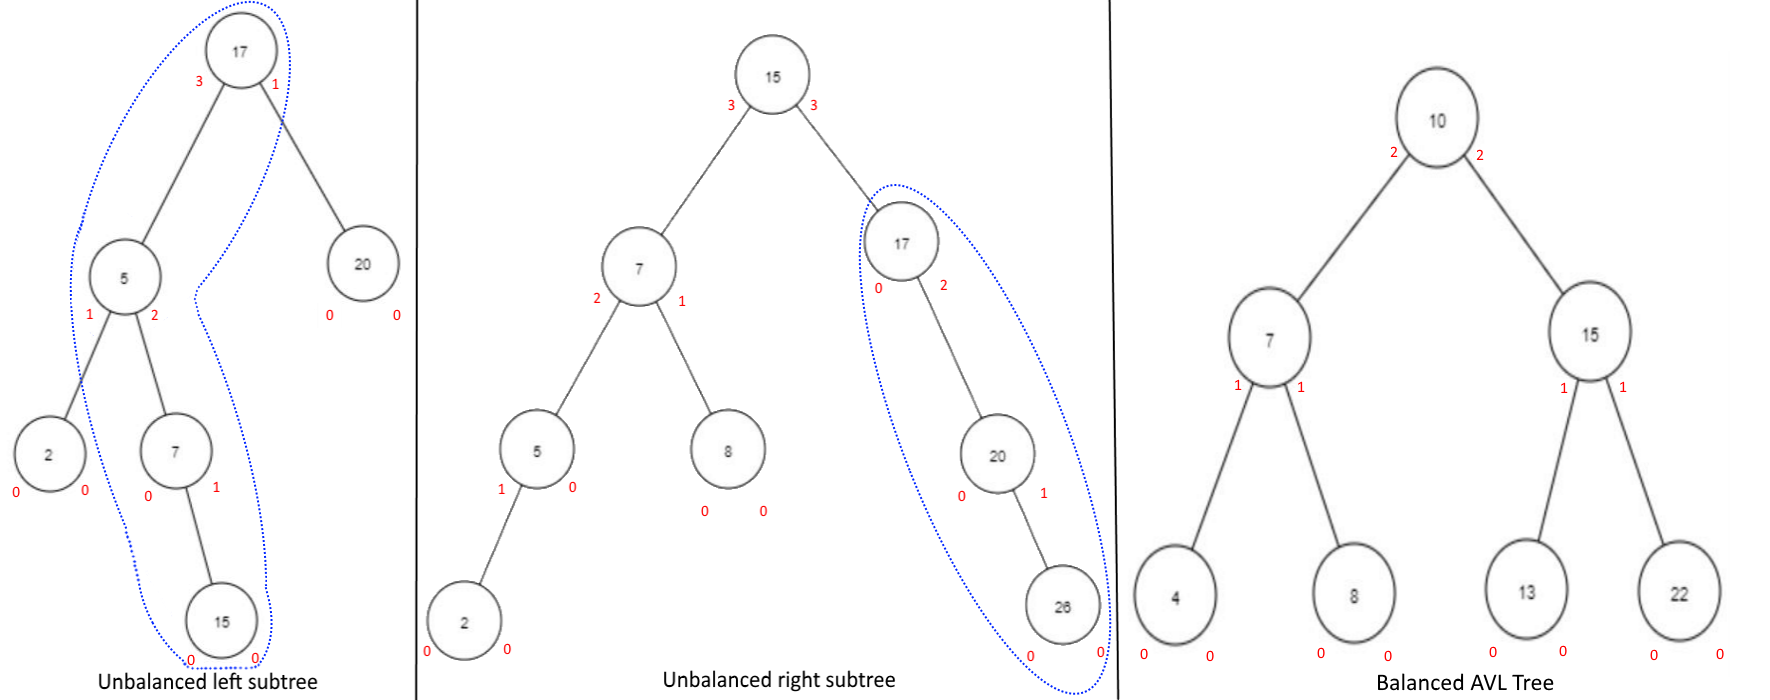
\includegraphics[width=\linewidth]{/trees/AVLTreesVer2.png}	
	\caption{The figure displays 2 unbalanced binary search trees and a fully balanced AVL tree. The left tree is a BST tree that has to many nodes in the left subtree.The center tree is a BST tree that has to many nodes in the right subtree. The tree to the right in the figure is a fully balanced Binary search tree, which makes it qualified as an AVL tree. \\The red letters represent the height of the node's children. The value is determined by how many nodes there are between the leaf nodes to the selected node. The blue dotted lines marks the subtree that breaks the AVL condition.}
	\label{fig:AVLTrees}
\end{figure}
